\documentclass[twoside]{book}

% Packages required by doxygen
\usepackage{fixltx2e}
\usepackage{calc}
\usepackage{doxygen}
\usepackage[export]{adjustbox} % also loads graphicx
\usepackage{graphicx}
\usepackage[utf8]{inputenc}
\usepackage{makeidx}
\usepackage{multicol}
\usepackage{multirow}
\PassOptionsToPackage{warn}{textcomp}
\usepackage{textcomp}
\usepackage[nointegrals]{wasysym}
\usepackage[table]{xcolor}

% Font selection
\usepackage[T1]{fontenc}
\usepackage[scaled=.90]{helvet}
\usepackage{courier}
\usepackage{amssymb}
\usepackage{sectsty}
\renewcommand{\familydefault}{\sfdefault}
\allsectionsfont{%
  \fontseries{bc}\selectfont%
  \color{darkgray}%
}
\renewcommand{\DoxyLabelFont}{%
  \fontseries{bc}\selectfont%
  \color{darkgray}%
}
\newcommand{\+}{\discretionary{\mbox{\scriptsize$\hookleftarrow$}}{}{}}

% Page & text layout
\usepackage{geometry}
\geometry{%
  a4paper,%
  top=2.5cm,%
  bottom=2.5cm,%
  left=2.5cm,%
  right=2.5cm%
}
\tolerance=750
\hfuzz=15pt
\hbadness=750
\setlength{\emergencystretch}{15pt}
\setlength{\parindent}{0cm}
\setlength{\parskip}{3ex plus 2ex minus 2ex}
\makeatletter
\renewcommand{\paragraph}{%
  \@startsection{paragraph}{4}{0ex}{-1.0ex}{1.0ex}{%
    \normalfont\normalsize\bfseries\SS@parafont%
  }%
}
\renewcommand{\subparagraph}{%
  \@startsection{subparagraph}{5}{0ex}{-1.0ex}{1.0ex}{%
    \normalfont\normalsize\bfseries\SS@subparafont%
  }%
}
\makeatother

% Headers & footers
\usepackage{fancyhdr}
\pagestyle{fancyplain}
\fancyhead[LE]{\fancyplain{}{\bfseries\thepage}}
\fancyhead[CE]{\fancyplain{}{}}
\fancyhead[RE]{\fancyplain{}{\bfseries\leftmark}}
\fancyhead[LO]{\fancyplain{}{\bfseries\rightmark}}
\fancyhead[CO]{\fancyplain{}{}}
\fancyhead[RO]{\fancyplain{}{\bfseries\thepage}}
\fancyfoot[LE]{\fancyplain{}{}}
\fancyfoot[CE]{\fancyplain{}{}}
\fancyfoot[RE]{\fancyplain{}{\bfseries\scriptsize Generated by Doxygen }}
\fancyfoot[LO]{\fancyplain{}{\bfseries\scriptsize Generated by Doxygen }}
\fancyfoot[CO]{\fancyplain{}{}}
\fancyfoot[RO]{\fancyplain{}{}}
\renewcommand{\footrulewidth}{0.4pt}
\renewcommand{\chaptermark}[1]{%
  \markboth{#1}{}%
}
\renewcommand{\sectionmark}[1]{%
  \markright{\thesection\ #1}%
}

% Indices & bibliography
\usepackage{natbib}
\usepackage[titles]{tocloft}
\setcounter{tocdepth}{3}
\setcounter{secnumdepth}{5}
\makeindex

% Hyperlinks (required, but should be loaded last)
\usepackage{ifpdf}
\ifpdf
  \usepackage[pdftex,pagebackref=true]{hyperref}
\else
  \usepackage[ps2pdf,pagebackref=true]{hyperref}
\fi
\hypersetup{%
  colorlinks=true,%
  linkcolor=blue,%
  citecolor=blue,%
  unicode%
}

% Custom commands
\newcommand{\clearemptydoublepage}{%
  \newpage{\pagestyle{empty}\cleardoublepage}%
}

\usepackage{caption}
\captionsetup{labelsep=space,justification=centering,font={bf},singlelinecheck=off,skip=4pt,position=top}

%===== C O N T E N T S =====

\begin{document}

% Titlepage & ToC
\hypersetup{pageanchor=false,
             bookmarksnumbered=true,
             pdfencoding=unicode
            }
\pagenumbering{alph}
\begin{titlepage}
\vspace*{7cm}
\begin{center}%
{\Large OO E\+X\+A\+M\+P\+LE }\\
\vspace*{1cm}
{\large Generated by Doxygen 1.8.13}\\
\end{center}
\end{titlepage}
\clearemptydoublepage
\pagenumbering{roman}
\tableofcontents
\clearemptydoublepage
\pagenumbering{arabic}
\hypersetup{pageanchor=true}

%--- Begin generated contents ---
\chapter{Hierarchical Index}
\section{Class Hierarchy}
This inheritance list is sorted roughly, but not completely, alphabetically\+:\begin{DoxyCompactList}
\item \contentsline{section}{Arquivo}{\pageref{class_arquivo}}{}
\item \contentsline{section}{Carrinho}{\pageref{class_carrinho}}{}
\item \contentsline{section}{Cliente}{\pageref{class_cliente}}{}
\begin{DoxyCompactList}
\item \contentsline{section}{Socio}{\pageref{class_socio}}{}
\end{DoxyCompactList}
\item \contentsline{section}{Inicio}{\pageref{class_inicio}}{}
\item \contentsline{section}{Livro}{\pageref{class_livro}}{}
\item \contentsline{section}{Recomenda}{\pageref{class_recomenda}}{}
\end{DoxyCompactList}

\chapter{Class Index}
\section{Class List}
Here are the classes, structs, unions and interfaces with brief descriptions\+:\begin{DoxyCompactList}
\item\contentsline{section}{\hyperlink{class_arquivo}{Arquivo} }{\pageref{class_arquivo}}{}
\item\contentsline{section}{\hyperlink{class_carrinho}{Carrinho} }{\pageref{class_carrinho}}{}
\item\contentsline{section}{\hyperlink{class_cliente}{Cliente} }{\pageref{class_cliente}}{}
\item\contentsline{section}{\hyperlink{class_inicio}{Inicio} }{\pageref{class_inicio}}{}
\item\contentsline{section}{\hyperlink{class_livro}{Livro} }{\pageref{class_livro}}{}
\item\contentsline{section}{\hyperlink{class_recomenda}{Recomenda} }{\pageref{class_recomenda}}{}
\item\contentsline{section}{\hyperlink{class_socio}{Socio} }{\pageref{class_socio}}{}
\end{DoxyCompactList}

\chapter{Class Documentation}
\hypertarget{class_arquivo}{}\section{Arquivo Class Reference}
\label{class_arquivo}\index{Arquivo@{Arquivo}}
\subsection*{Public Member Functions}
\begin{DoxyCompactItemize}
\item 
\mbox{\Hypertarget{class_arquivo_a85d0577393ab9d2293ca837fe3c0d11a}\label{class_arquivo_a85d0577393ab9d2293ca837fe3c0d11a}} 
string {\bfseries retorna\+\_\+linha} (string path, int linha)
\item 
\mbox{\Hypertarget{class_arquivo_a3a57b58a5ae3609ead87eef74c84cab2}\label{class_arquivo_a3a57b58a5ae3609ead87eef74c84cab2}} 
void {\bfseries modifica\+\_\+preco} (string path, double novo\+\_\+preco)
\item 
\mbox{\Hypertarget{class_arquivo_a13175f4b22c398c3982a073dece8b2a7}\label{class_arquivo_a13175f4b22c398c3982a073dece8b2a7}} 
void {\bfseries modifica\+\_\+quantidade} (string path, int nova\+\_\+quantidade)
\end{DoxyCompactItemize}


The documentation for this class was generated from the following files\+:\begin{DoxyCompactItemize}
\item 
inc/arquivo.\+hpp\item 
src/arquivo.\+cpp\end{DoxyCompactItemize}

\hypertarget{class_carrinho}{}\section{Carrinho Class Reference}
\label{class_carrinho}\index{Carrinho@{Carrinho}}
\subsection*{Public Member Functions}
\begin{DoxyCompactItemize}
\item 
\mbox{\Hypertarget{class_carrinho_a485ede9af50b4d6f0ec09a733188c84f}\label{class_carrinho_a485ede9af50b4d6f0ec09a733188c84f}} 
bool {\bfseries verifica\+\_\+quantidade} (vector$<$ string $>$ livro)
\item 
\mbox{\Hypertarget{class_carrinho_ab9ac6c0fd232050fa9ff7a550cf1c775}\label{class_carrinho_ab9ac6c0fd232050fa9ff7a550cf1c775}} 
void {\bfseries total\+\_\+carrinho} (vector$<$ string $>$ livro, string cpf)
\item 
\mbox{\Hypertarget{class_carrinho_a1425fb2e6c6d2c976cab8669c9086cc5}\label{class_carrinho_a1425fb2e6c6d2c976cab8669c9086cc5}} 
void {\bfseries situacao\+\_\+carrinho} (vector$<$ string $>$ livro)
\item 
\mbox{\Hypertarget{class_carrinho_ac0361c2825364a975486080e045d5f2a}\label{class_carrinho_ac0361c2825364a975486080e045d5f2a}} 
void {\bfseries remove\+\_\+quantidade} (vector$<$ string $>$ livro)
\item 
\mbox{\Hypertarget{class_carrinho_ad50c097d0445c57ed4984bb70ce36b88}\label{class_carrinho_ad50c097d0445c57ed4984bb70ce36b88}} 
void {\bfseries salva\+\_\+produtos} (vector$<$ string $>$ livro, string cpf)
\end{DoxyCompactItemize}


The documentation for this class was generated from the following files\+:\begin{DoxyCompactItemize}
\item 
inc/carrinho.\+hpp\item 
src/carrinho.\+cpp\end{DoxyCompactItemize}

\hypertarget{class_cliente}{}\section{Cliente Class Reference}
\label{class_cliente}\index{Cliente@{Cliente}}
Inheritance diagram for Cliente\+:\begin{figure}[H]
\begin{center}
\leavevmode
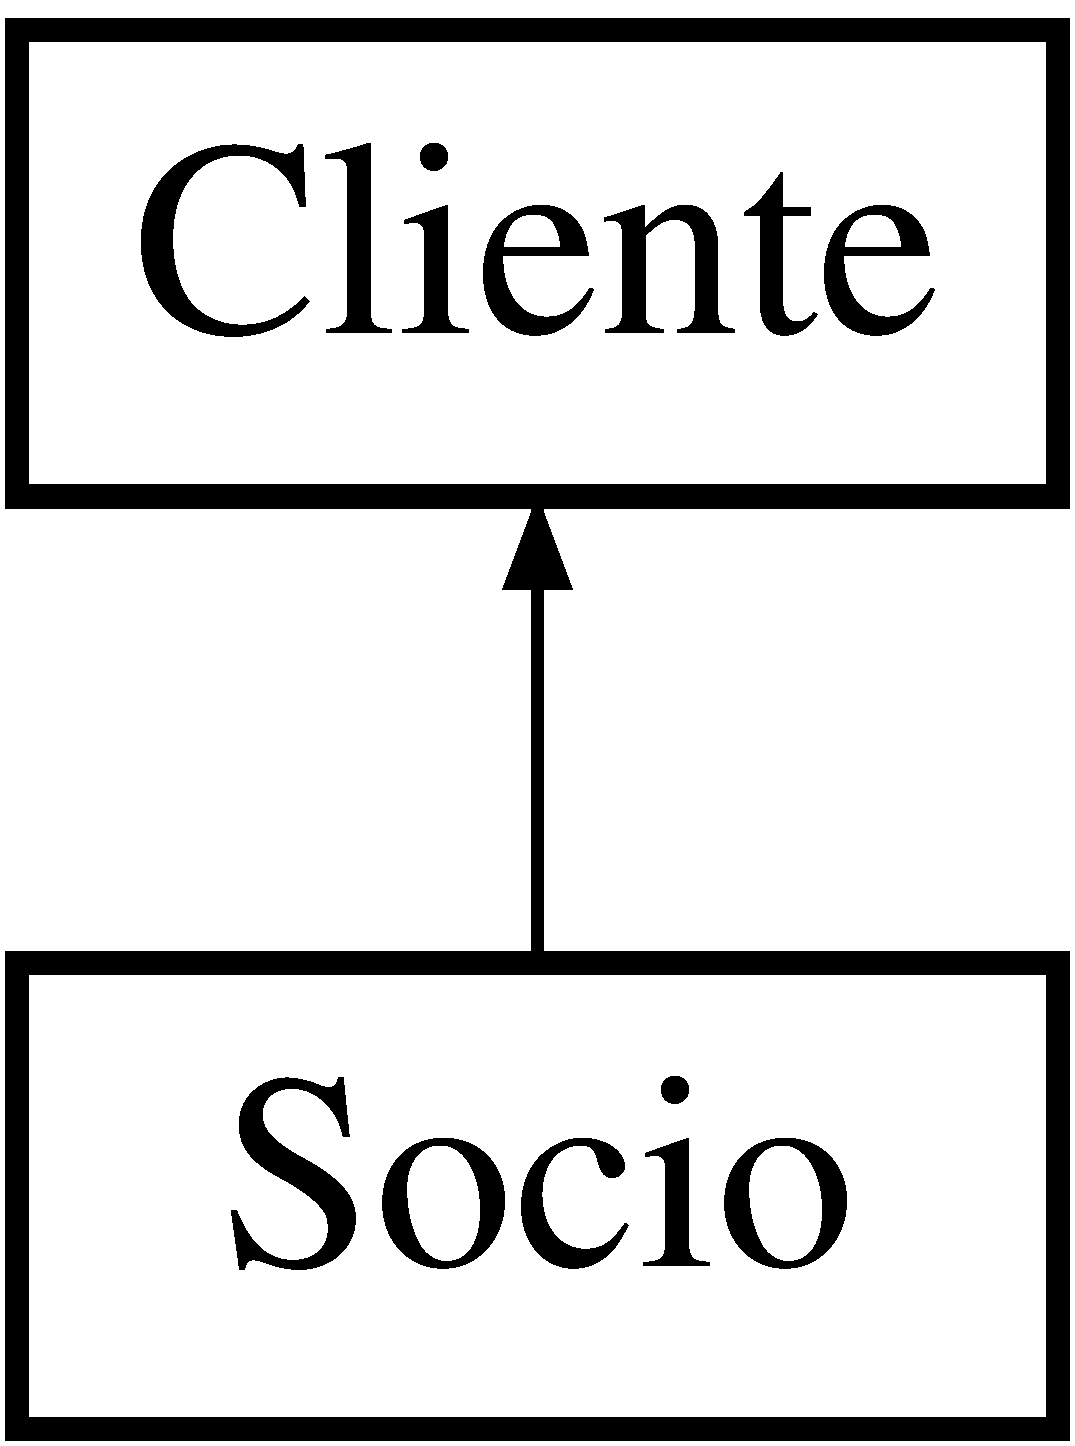
\includegraphics[height=2.000000cm]{class_cliente}
\end{center}
\end{figure}
\subsection*{Public Member Functions}
\begin{DoxyCompactItemize}
\item 
\mbox{\Hypertarget{class_cliente_a7b2229475422c8e630d3ef18942fbf0d}\label{class_cliente_a7b2229475422c8e630d3ef18942fbf0d}} 
{\bfseries Cliente} (string nome, string cpf, string email, string telefone)
\item 
\mbox{\Hypertarget{class_cliente_ae25672e2caaad4b621d868519747137b}\label{class_cliente_ae25672e2caaad4b621d868519747137b}} 
string {\bfseries get\+\_\+nome} ()
\item 
\mbox{\Hypertarget{class_cliente_a7cc80f947a4e62a7623e6c3bb0cb0ef0}\label{class_cliente_a7cc80f947a4e62a7623e6c3bb0cb0ef0}} 
void {\bfseries set\+\_\+nome} (string nome)
\item 
\mbox{\Hypertarget{class_cliente_a093f55c599f35d80f0dffc2353414950}\label{class_cliente_a093f55c599f35d80f0dffc2353414950}} 
string {\bfseries get\+\_\+cpf} ()
\item 
\mbox{\Hypertarget{class_cliente_a2d3a1e3d2ee79f4f88ceaa8a8757f87d}\label{class_cliente_a2d3a1e3d2ee79f4f88ceaa8a8757f87d}} 
void {\bfseries set\+\_\+cpf} (string cpf)
\item 
\mbox{\Hypertarget{class_cliente_a4ee3af001aef36ace0f6f07611d6d18b}\label{class_cliente_a4ee3af001aef36ace0f6f07611d6d18b}} 
string {\bfseries get\+\_\+email} ()
\item 
\mbox{\Hypertarget{class_cliente_af37b3b0d7bc542523dc077649842516e}\label{class_cliente_af37b3b0d7bc542523dc077649842516e}} 
void {\bfseries set\+\_\+email} (string email)
\item 
\mbox{\Hypertarget{class_cliente_aff1eb27693522ea7e66bba4496fdbca4}\label{class_cliente_aff1eb27693522ea7e66bba4496fdbca4}} 
string {\bfseries get\+\_\+telefone} ()
\item 
\mbox{\Hypertarget{class_cliente_a3087f1a2e20ca52e4bd16ea3156e0747}\label{class_cliente_a3087f1a2e20ca52e4bd16ea3156e0747}} 
void {\bfseries set\+\_\+telefone} (string telefone)
\item 
\mbox{\Hypertarget{class_cliente_a6818bb286b8fbaaf6056fab6fb2c24ec}\label{class_cliente_a6818bb286b8fbaaf6056fab6fb2c24ec}} 
bool {\bfseries verifica\+\_\+cliente} (string cpf)
\item 
\mbox{\Hypertarget{class_cliente_a57de17bbebc2b90e1732cdbbd9b15e30}\label{class_cliente_a57de17bbebc2b90e1732cdbbd9b15e30}} 
string {\bfseries verifica\+\_\+cpf} ()
\item 
\mbox{\Hypertarget{class_cliente_a62328e77ee9e9621db1effdb30d44a9f}\label{class_cliente_a62328e77ee9e9621db1effdb30d44a9f}} 
void {\bfseries imprime\+\_\+dados} ()
\item 
\mbox{\Hypertarget{class_cliente_a0c37adb2060050740b7b330fbffdd134}\label{class_cliente_a0c37adb2060050740b7b330fbffdd134}} 
string {\bfseries salva\+\_\+dados} ()
\end{DoxyCompactItemize}


The documentation for this class was generated from the following files\+:\begin{DoxyCompactItemize}
\item 
inc/cliente.\+hpp\item 
src/cliente.\+cpp\end{DoxyCompactItemize}

\hypertarget{class_inicio}{}\section{Inicio Class Reference}
\label{class_inicio}\index{Inicio@{Inicio}}
\subsection*{Public Member Functions}
\begin{DoxyCompactItemize}
\item 
\mbox{\Hypertarget{class_inicio_a1b19189e2b26727c835afa465be7a4d2}\label{class_inicio_a1b19189e2b26727c835afa465be7a4d2}} 
void {\bfseries modo\+\_\+inicio} ()
\item 
\mbox{\Hypertarget{class_inicio_aefd6c9cea6dd76c9c3953c854ad47483}\label{class_inicio_aefd6c9cea6dd76c9c3953c854ad47483}} 
void {\bfseries modo\+\_\+venda} ()
\item 
\mbox{\Hypertarget{class_inicio_a6c81a17a924bbcf3b2dec6251530149d}\label{class_inicio_a6c81a17a924bbcf3b2dec6251530149d}} 
void {\bfseries modo\+\_\+estoque} ()
\item 
\mbox{\Hypertarget{class_inicio_a23f98e4d158e53d0807cd747b0944d52}\label{class_inicio_a23f98e4d158e53d0807cd747b0944d52}} 
void {\bfseries modo\+\_\+recomenda} ()
\end{DoxyCompactItemize}


The documentation for this class was generated from the following files\+:\begin{DoxyCompactItemize}
\item 
inc/inicio.\+hpp\item 
src/inicio.\+cpp\end{DoxyCompactItemize}

\hypertarget{class_livro}{}\section{Livro Class Reference}
\label{class_livro}\index{Livro@{Livro}}
\subsection*{Public Member Functions}
\begin{DoxyCompactItemize}
\item 
\mbox{\Hypertarget{class_livro_a1de7a3e9ab043a18e07ed5de2a69a703}\label{class_livro_a1de7a3e9ab043a18e07ed5de2a69a703}} 
{\bfseries Livro} (string nome\+\_\+livro, int codigo\+\_\+livro, string categoria, double valor, int quantidade)
\item 
\mbox{\Hypertarget{class_livro_aef9feeb00689ed50335053cf51f89c93}\label{class_livro_aef9feeb00689ed50335053cf51f89c93}} 
string {\bfseries get\+\_\+nome\+\_\+livro} ()
\item 
\mbox{\Hypertarget{class_livro_aa929cc65370f6250b69eb437e8039f19}\label{class_livro_aa929cc65370f6250b69eb437e8039f19}} 
void {\bfseries set\+\_\+nome\+\_\+livro} (string nome\+\_\+livro)
\item 
\mbox{\Hypertarget{class_livro_a2bf1a0fcaa06b753903f2f07f7373bf6}\label{class_livro_a2bf1a0fcaa06b753903f2f07f7373bf6}} 
int {\bfseries get\+\_\+codigo\+\_\+livro} ()
\item 
\mbox{\Hypertarget{class_livro_ab7101b172aae2011117b235d4abfa58f}\label{class_livro_ab7101b172aae2011117b235d4abfa58f}} 
void {\bfseries set\+\_\+codigo\+\_\+livro} (int codigo\+\_\+livro)
\item 
\mbox{\Hypertarget{class_livro_acc54282e8093f3f3628cf291ebbfce7f}\label{class_livro_acc54282e8093f3f3628cf291ebbfce7f}} 
string {\bfseries get\+\_\+categoria} ()
\item 
\mbox{\Hypertarget{class_livro_a1c6fea76f1732e959720971c9791d125}\label{class_livro_a1c6fea76f1732e959720971c9791d125}} 
void {\bfseries set\+\_\+categoria} (string categoria)
\item 
\mbox{\Hypertarget{class_livro_ad3289981dc5bf28e927d769d2e44af28}\label{class_livro_ad3289981dc5bf28e927d769d2e44af28}} 
double {\bfseries get\+\_\+valor} ()
\item 
\mbox{\Hypertarget{class_livro_a2a35d394858c7a432ed483994288fad8}\label{class_livro_a2a35d394858c7a432ed483994288fad8}} 
void {\bfseries set\+\_\+valor} (double valor)
\item 
\mbox{\Hypertarget{class_livro_ade24f1e83c1b0bcb26845e4dc7e2112b}\label{class_livro_ade24f1e83c1b0bcb26845e4dc7e2112b}} 
int {\bfseries get\+\_\+quantidade} ()
\item 
\mbox{\Hypertarget{class_livro_a862ad3d2c1d7754e347b84f633b0cd58}\label{class_livro_a862ad3d2c1d7754e347b84f633b0cd58}} 
void {\bfseries set\+\_\+quantidade} (int quantidade)
\item 
\mbox{\Hypertarget{class_livro_a0697d3698bca92189fa6c3cce8dc8e39}\label{class_livro_a0697d3698bca92189fa6c3cce8dc8e39}} 
void {\bfseries lista\+\_\+livro} (string categoria)
\item 
\mbox{\Hypertarget{class_livro_a50ab2684b4334261df00886c755cfd9d}\label{class_livro_a50ab2684b4334261df00886c755cfd9d}} 
void {\bfseries lista\+\_\+categoria} ()
\item 
\mbox{\Hypertarget{class_livro_afa685bdc099394ffd94e0f70ef6de500}\label{class_livro_afa685bdc099394ffd94e0f70ef6de500}} 
string {\bfseries verifica\+\_\+categoria} ()
\item 
\mbox{\Hypertarget{class_livro_a27d660e47fe333768d96ed7186923c74}\label{class_livro_a27d660e47fe333768d96ed7186923c74}} 
int {\bfseries verifica\+\_\+livro} (string categoria)
\item 
\mbox{\Hypertarget{class_livro_ad8bf1a52295d2c5b7f696c4956f43e7c}\label{class_livro_ad8bf1a52295d2c5b7f696c4956f43e7c}} 
void {\bfseries imprime\+\_\+dados} ()
\item 
\mbox{\Hypertarget{class_livro_abb1d98a0c48f6bde82fc31dbcf1fe38d}\label{class_livro_abb1d98a0c48f6bde82fc31dbcf1fe38d}} 
string {\bfseries salva\+\_\+dados} ()
\end{DoxyCompactItemize}


The documentation for this class was generated from the following files\+:\begin{DoxyCompactItemize}
\item 
inc/livro.\+hpp\item 
src/livro.\+cpp\end{DoxyCompactItemize}

\hypertarget{class_recomenda}{}\section{Recomenda Class Reference}
\label{class_recomenda}\index{Recomenda@{Recomenda}}
\subsection*{Public Member Functions}
\begin{DoxyCompactItemize}
\item 
\mbox{\Hypertarget{class_recomenda_ac095a8cd9053b5e88808ff56198e4fd1}\label{class_recomenda_ac095a8cd9053b5e88808ff56198e4fd1}} 
void {\bfseries recomendados} (string cpf)
\end{DoxyCompactItemize}


The documentation for this class was generated from the following files\+:\begin{DoxyCompactItemize}
\item 
inc/recomenda.\+hpp\item 
src/recomenda.\+cpp\end{DoxyCompactItemize}

\hypertarget{class_socio}{}\section{Socio Class Reference}
\label{class_socio}\index{Socio@{Socio}}
Inheritance diagram for Socio\+:\begin{figure}[H]
\begin{center}
\leavevmode
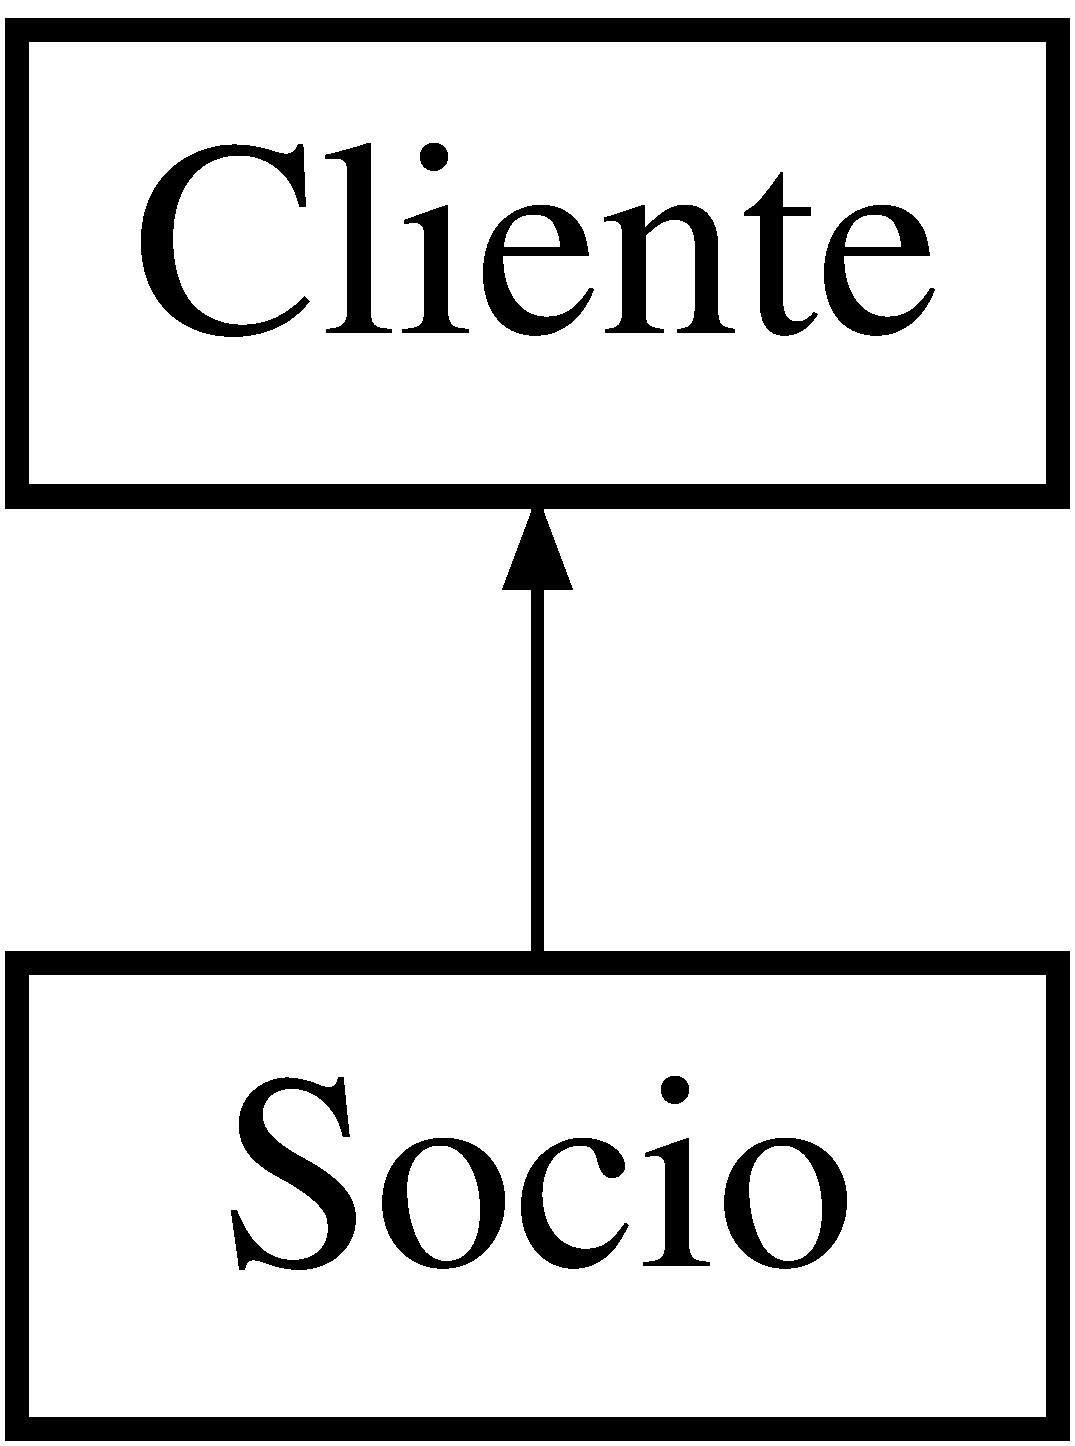
\includegraphics[height=2.000000cm]{class_socio}
\end{center}
\end{figure}
\subsection*{Public Member Functions}
\begin{DoxyCompactItemize}
\item 
\mbox{\Hypertarget{class_socio_a20417da9fca1fedf8d6526bb5726d1c4}\label{class_socio_a20417da9fca1fedf8d6526bb5726d1c4}} 
{\bfseries Socio} (string nome, string cpf, string email, string telefone)
\item 
\mbox{\Hypertarget{class_socio_a485c34043429f469752e2396b54a9494}\label{class_socio_a485c34043429f469752e2396b54a9494}} 
bool {\bfseries verifica\+\_\+socio} (string socio)
\item 
\mbox{\Hypertarget{class_socio_a8d0dba2699f6cf66b6c5b5bb6dc97853}\label{class_socio_a8d0dba2699f6cf66b6c5b5bb6dc97853}} 
double {\bfseries desconto\+\_\+socio} (double valor)
\end{DoxyCompactItemize}


The documentation for this class was generated from the following files\+:\begin{DoxyCompactItemize}
\item 
inc/socio.\+hpp\item 
src/socio.\+cpp\end{DoxyCompactItemize}

%--- End generated contents ---

% Index
\backmatter
\newpage
\phantomsection
\clearemptydoublepage
\addcontentsline{toc}{chapter}{Index}
\printindex

\end{document}
